\documentclass{beamer}
\begin{document}
    \begin{frame}
        Course Overview:
        \begin{itemize}
            \item The first half of the course will focus on the basics of Python programming, data manipulation, and visualization.
            \item The course is structured with a heavy emphasis on lectures in the beginning before a gradual shift to a lab/exercise heave session.
            \item The first half of the course will be taught exclusively in English.
            \item But assignment/coursework can be submitted in either English or German.
            \item The first half of the course will graded based on the assignment/coursework given at the transition between the first and second half of the course.
        \end{itemize}
    \end{frame}
        
    % \subsection{Warum auf Englisch?}
    \begin{frame}
        \frametitle{Warum wir diesen datenwissenschaftlichen Kurs auf Englisch unterrichten}
        \begin{itemize}
            \item Die meisten Programmiersprachen, einschließlich Python, sind auf Englisch entwickelt
            \item Englisch ist die internationale Sprache der Datenverarbeitung und Informationstechnologie
            \item Die gemeinsame Englische Sprache fördert die Zusammenarbeit und Kommunikation weltweit
            \item Einige unserer Dozenten \& Tutoren sprechen nur Englisch weil wir ein internationaler Forschungsstandort sind.
        \end{itemize}
        % \begin{center}
        % \end{center}
    \end{frame}
        
    \begin{frame}
        \frametitle{Datenwissenschaftliche Ressourcen sind auf Englisch}
        \begin{center}
            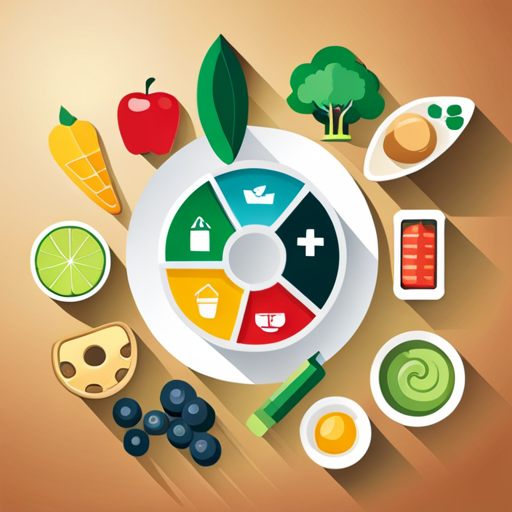
\includegraphics[width=0.25\textwidth]{figures/data-science-resources-english}
        \end{center}
        \begin{itemize}
            \item Die meisten Lehrmaterialien, Tutorials und Online-Kurse zur Datenwissenschaft sind auf Englisch verfügbar
            \item Die englische Fachliteratur bietet den aktuellsten Stand der Forschung und Technologie
            \item Nutzung von Englisch erleichtert den Zugang zu Ressourcen und ermöglichen ein schnelleres Lernen
        \end{itemize}
    \end{frame}
        
    \begin{frame}
        \frametitle{Datenwissenschaftlicher Code ist auf Englisch}
        \begin{center}
            
\includegraphics[width=0.33\textwidth]{figures/healthcare-analytics.png}
        \end{center}
        \begin{itemize}
            \item Die meisten Open-Source-Projekte, Software-Bibliotheken und Codebeispiele sind auf Englisch geschrieben
            \item Englischsprachiger Code ist oft leichter zu verstehen, zu verwenden und kürzer
            \item Die Verwendung von Englisch für die Programmierung fördert die Wiederverwendbarkeit und Zusammenarbeit weltweit
        \end{itemize}
        % \begin{center}
        
        % \end{center}
    \end{frame}
    \subsection{Introduction to Data Science \& Big Data} 
    \begin{frame}
        \frametitle{Introduction to Data Science \& Big Data}
        \begin{itemize}
            \item Data science is a powerful tool for analyzing and understanding complex datasets
            \item Applications in food, nutrition, and Health are vast and fast-growing
            \item Opportunities to optimize designs, improve decision-making, better health outcomes, and overall well-being
        \end{itemize}
    \end{frame}
        
    \begin{frame}
        \frametitle{Improving Nutrition \& Dietary Recommendations}
        \begin{center}
            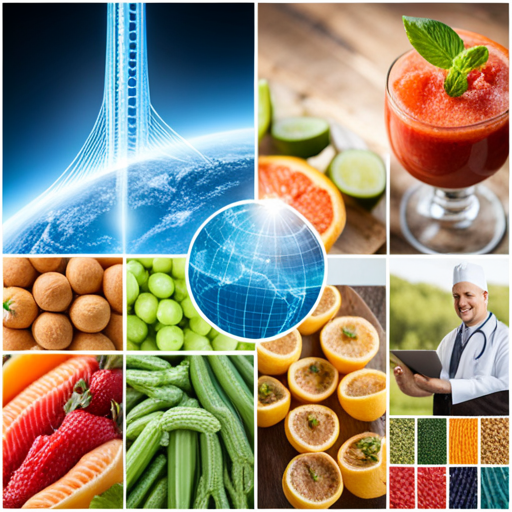
\includegraphics[width=0.33\textwidth]{figures/nutrition-data-science}
        \end{center}
        \begin{itemize}
            \item Analyzing food consumption data to develop personalized dietary plans
            \item Identifying nutrient deficiencies and optimizing nutrient intake
            \item Evaluating the impact of diet on health outcomes and disease prevention
        \end{itemize}
    \end{frame}
        
    \begin{frame}
        \frametitle{Advancing Health \& Disease Prevention}
        \begin{center}
            
\includegraphics[width=0.33\textwidth]{figures/healthcare-data-science.png}
        \end{center}
        \begin{itemize}
            \item Predicting and preventing disease outbreaks using data analytics
            \item Analyzing electronic health records to improve patient care
            \item Discovering patterns in genetic data to advance personalized medicine
        \end{itemize}
    \end{frame}
        
    \begin{frame}
        \frametitle{What is Big Data?}
        \begin{itemize}
            \item Big Data refers to a set of data that contain great variety, velocity, and volume.
            \item Due to the volume and complexity of the data, traditional data processing software could not manage them.
            \item Big Data often contains various heterogeneous data types such as text, images, and videos.
        \end{itemize}
    \end{frame}
        
    \begin{frame}
        \frametitle{Why Big Data?}
        \begin{itemize}
            \item Currently, 140 Zettabytes of data are being produced and consumed by the world.
            \item Growing applications in both the Healthcare and Food/Nutrition segment.
            \item Big Data offers greater statistical power and insight.
        \end{itemize}
    \end{frame}
        
    \subsection{Why Learn Python?}
    \subsubsection{Python: The Leading Language for Data Science}
    \begin{frame}
        \frametitle{Python: The Leading Language for Data Science}
        \begin{center}
            
\includegraphics[width=0.3\textwidth]{figures/Python-Symbol}
        \end{center}
        \begin{itemize}
            \item A high-level, interpreted programming language
            \item Developed by Guido van Rossum in the late 1980s
            \item Emphasizes readability, simplicity, versatility, and easy-to-learn mantra.
            \item Widely used in various fields, such as data science, web development, and scientific computing.
            \item Rich ecosystem of libraries and tools for data analysis and visualization (including helpful forums).
        \end{itemize}
    \end{frame}
        
        
    \subsubsection{Python Libraries for Data Science}
    \begin{frame}
        \frametitle{Python Libraries for Data Science}
        \begin{block}{Libraries}
            A software library is a collection of pre-written code, functions, or routines that developers can use to perform everyday tasks, solve problems, or implement specific features. Libraries are designed to be reusable and modular, allowing developers to save time and effort by avoiding the need to (re)write code from scratch.
        \end{block}
        
        \begin{itemize}
            \item NumPy: Numerical computing and array manipulation
            \item Pandas: Data manipulation and analysis
            \item Matplotlib: Data visualization and plotting
            \item Scikit-learn: Machine learning and data mining
            \item TensorFlow and PyTorch: Deep learning and neural networks
        \end{itemize}
    \end{frame}
        
        
    \subsubsection{Community and Career Opportunities}
    \begin{frame}
        \frametitle{Community and Career Opportunities}
        \begin{itemize}
            \item A Vibrant Python community offers support, resources, and collaboration
            \item High demand for Python developers and data scientists in various industries
            \item Python skills can open doors to exciting career opportunities for careers involving data analysis or data creation
        \end{itemize}
    \end{frame}
        
    \subsubsection{Interesting Python Tool -- Google Colab}
    \begin{frame}
        \frametitle{What is Google Colab?}
        \begin{itemize}
            \item Google Colab is a free, cloud-based Jupyter Notebook environment
            %\item Offers GPU and TPU support for faster computation
            \item Ideal for machine learning, data analysis, and collaboration
            \item No setup required runs entirely in your web browser
            \item Visit \url{https://colab.research.google.com/} to access Google Colab
            \item Sign in with your Google account
            \item Create a new notebook by clicking on File' $\rightarrow$ New notebook'
            \item Open an existing notebook from Google Drive or upload a local file
        \end{itemize}
    \end{frame}
\end{document}